\section{Design and Implementation}
LibSmoke is composed essentially, as told before, by SKNX and AES.\par
\vspace{5mm}
\textbf{Secure KNX - }Allows the user to create the \emph{backend} connection between different devices, in particular in this paper/project we have considered the LinuxTCP one. It includes also a \emph{pktwrapper} that handles the packets exchange : splitting data in pkts of 15 bytes payload and recomposing next them together. There are also available multiple KeyExchange algorithms that allows to calculate a shared key; we have here test the \emph{mka} (Multi-party Key Agreement Algorithm).\par
\vspace{5mm}
\textbf{AES256\_CTR - }Given that \emph{mka} returns a key of 32 bytes we choose AES256, but in the \emph{AES Library} there are also available AES128 and AES192. It includes all the implementations of AES ECB, CTR and CBC, in particular we use CTR cause it also provides padding.\par
\vspace{5mm}
Given this background we decide to split LibSmoke in 2 classes : ClientSmoke and ServerSmoke.

\vspace{0.5cm}
\begin{figure}[h]
	\centering
	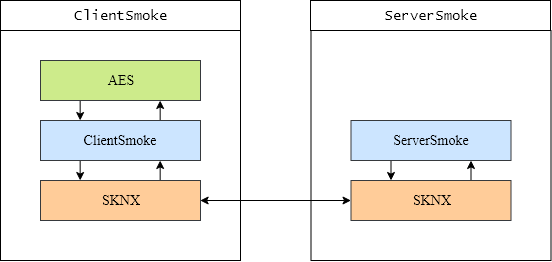
\includegraphics[scale=0.7]{Images/Diagrams/Architecture}
	\caption{LibSmoke Architecture}
\end{figure}
\vspace{0.2cm}

\newpage
\subsection{ClientSmoke}
Initialized by devices that needs to send and receive pkts, given also the functionality to encrypt and decrypt data with the encryption algorithm [AES256\_CTR].

\vspace{5mm}
\begin{lstlisting}[language=C++, caption={ClientSmoke}]
/**
* Class of Libsmoke Client.
*
* @param KeyAlgorithm - is the KeyExchange Algorithm
*			needed for SKNX to generate the key.
* @param PORT - is the PORT used by sockets.
* @param numClients - is the #Clients connected.
*/
template<typename KeyAlgorithm, uint16_t PORT,
			size_t numClients>
class ClientSmoke {
public:
/**
* Constructor of Libsmoke Client.
*
* @param addr const char* - is a pointer to the IP
*			to which socket client has to connect.
*/
ClientSmoke(const char *addr);

/**
* Initializes _backend and sknx.
* When sknx is ONLINE retrieves the KeyAlgorithm.
*
* \return     TRUE - if all initializations are completed
*			succesfully and key is retrieved.
*             FALSE - if there's an error on initialization
*			or key retrieving.
*/
bool init();
\end{lstlisting}

\newpage
\begin{lstlisting}[language=C++, caption={ClientSmoke}]
/**
* Uses pktwrapper in order to get the oldest pkt received
*			from other clients.
* It decrypts the body using AES_CTR with the shared key
*			of the client.
*
* @param data KNX::pkt_t& - pointer to a pkt that the method
*			uses to pass the oldest recieved one.
* @return TRUE - if there is actually a recieved pkt in the
*			queue of pktwrapper.
*         FALSE - if no pkt is received.
*/
bool receive(KNX::pkt_t &data);

/**
* Uses pktwrapper in order to send data (buf), with a specific
*	length (len) and command (cmd),
*	to a specific destination (dest).
* It encrypts the body using AES_CTR with the shared key
*	of the client.
*
* @param dest - the destination of the data.
* @param cmd - the command to send to the client(s).
* @param buf - the data, if there are, to send.
* @param len - the length of the data (can be also 0).
*/
void send(uint16_t dest, uint8_t cmd, uint8_t *buf,
uint16_t len);
\end{lstlisting}
\vspace{0.7cm}

\textbf{NB : }the user can choose the KeyExchange Algorithm from the ones already implemented and available inside the SKNX library.

\newpage
\subsection{ServerSmoke}
It's main features are to instantiate socket connections and broadcast the received pkts from the clients.

\begin{lstlisting}[language=C++, caption={ServerSmoke}]
class ServerSmoke{
public:
/**
* Constructor of Libsmoke Server.
* Sets _ready to false in order to say that the server
*	is not yet initialized.
*/
ServerSmoke() : _ready(false);

/**
* Checks if the server is already initialized.
* If not, creates the socket with the given IP and PORT.
*
* @param addr - IP addr of the socket to create.
* @param port - PORT of the socket to create.
* @return TRUE - if socket is created with no errors
*	and is listening.
*         FALSE - otherwise.
*/
bool init(const char *addr, int port);

/**
* Handles connections : registering the new ones
*	or deleting the closed ones.
* Also used to broadcast messages to all connected clients.
*/
void run();

/**
* Destructor of Libsmoke Server.
* Used to close all sockets and clear the vector
*	of the registered clients.
* Sets also _ready to false, so the server
*	can be initialized again.
*/
-ServerSmoke();
\end{lstlisting}

\newpage
\subsection{Instructions to Use}
\vspace{0.5cm}
\begin{itemize}
	\setlength{\leftskip}{0.5cm}
	\item ClientSmoke : '\emph{\#include "libsmoke\_client.h"}'
	\item ServerSmoke : '\emph{\#include "libsmoke\_server.h"}'
\end{itemize}
\vspace{0.2cm}

\textbf{NB : }in the repository is available also a `tests` directory, where inside can find `client\_test` and `server\_test`, that show how to use the library.